% --------------------------------------------------------------
% Basic LaTeX template for homework assignments.
% COMS W4701 - Artificial Intelligence
% --------------------------------------------------------------
\documentclass[11pt]{article}

\usepackage[margin=1in]{geometry}
\usepackage{amsmath,amsthm,amssymb}
\usepackage{tabularx}
\usepackage[T1]{fontenc}
\usepackage{enumerate}
\usepackage[]{forest}
\usepackage{float}
\restylefloat{table}
\graphicspath{ {./img/} }

\forestset{.style={for tree=
{parent anchor=south, child anchor=north,align=center,inner sep=2pt}}}

\begin{document}

%           Your solutions start below this line
% --------------------------------------------------------------

\title{COMS W4119: Computer Networks\\
       Homework 3}
\author{Jackson Chen (jc4697)} % replace with your name and UNI
\maketitle

\section*{Principles of Transport and Reliable Data Transfer}
  \begin{enumerate}[(a)]
    \item
      \begin{enumerate}[(i)]
        \item A timeout based retransmission mechanism can deal with both losses in
          sending packets and receiving ACK's. If the timer times out when waiting for ACK
          from receiver, it will just resend the packet. This will cover both situations
          where packets sent or ACKs received are lost. In addition, if the packet wasn't
          actually lost and it just took exceptionally long for the receiver to respond with
          the ACK, the packets are numbered and duplicate packets can be dealt with.
        \item
          The receiver FSM of rdt3.0 should be exactly the same as that of rdt2.2

          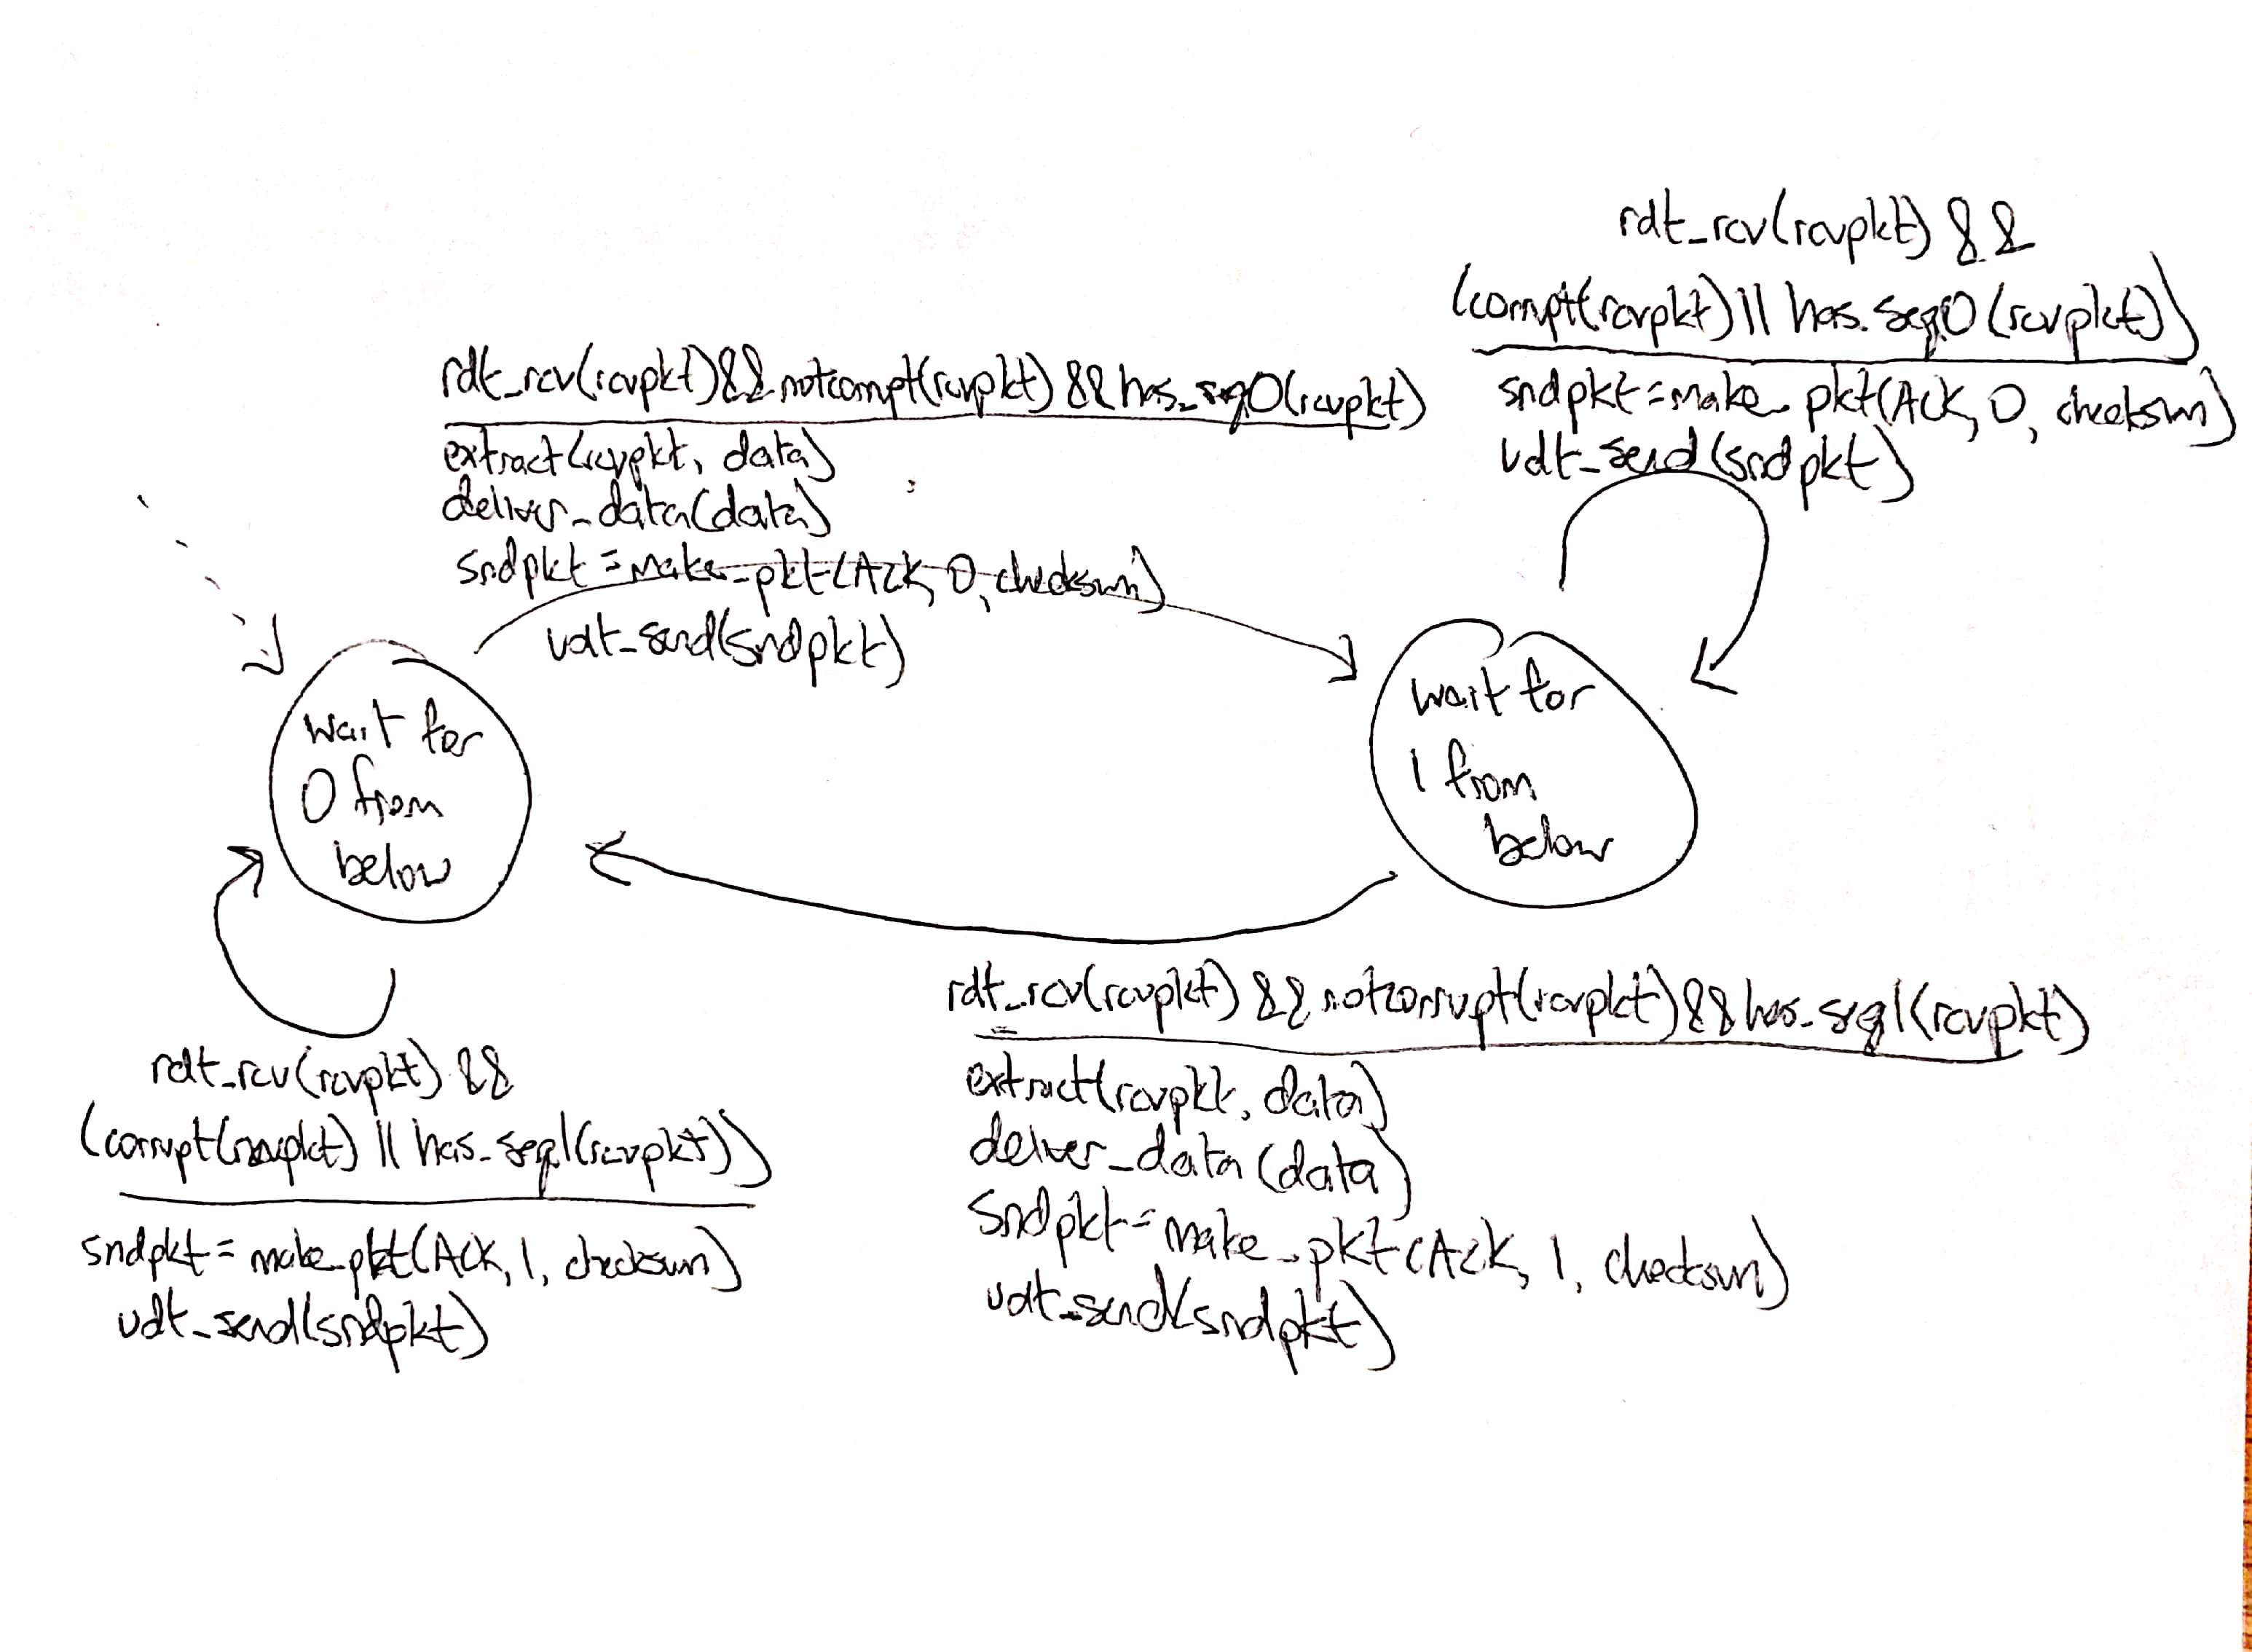
\includegraphics[width=15cm]{q1pa}
      \end{enumerate}
    \item
      The underlined numbers are the packets that are within the window, and the
      bolded packets are the ones sent on either side.

      Go Back N:

      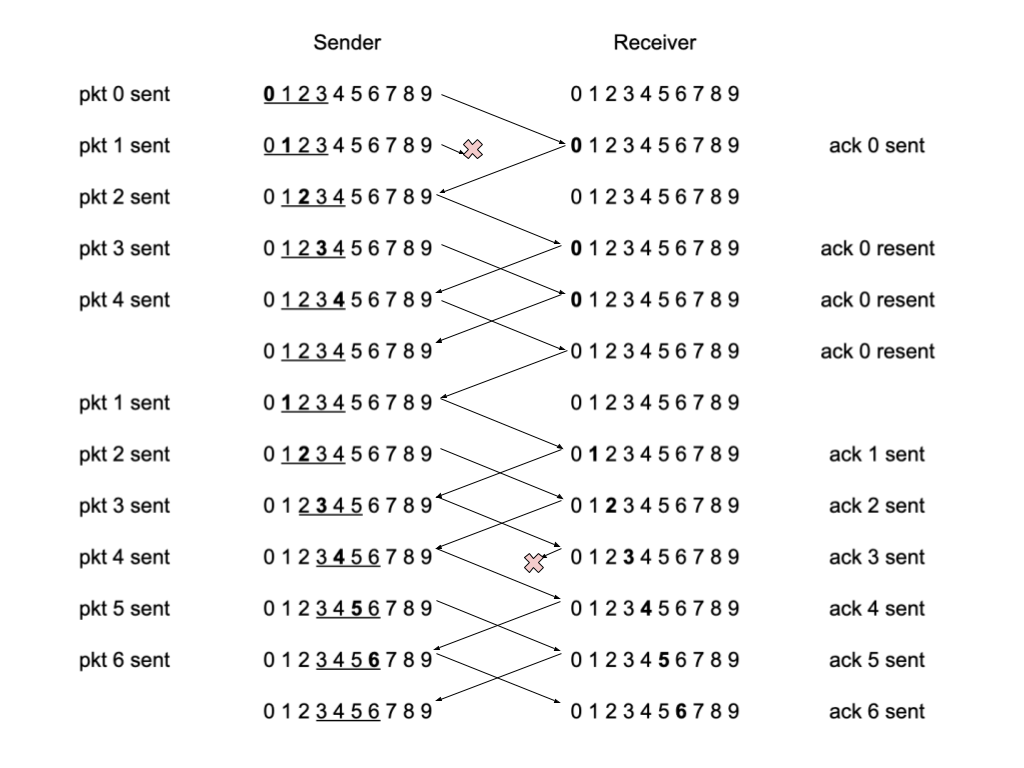
\includegraphics[width=15cm]{q1pb1}

      Selective Repeat:

      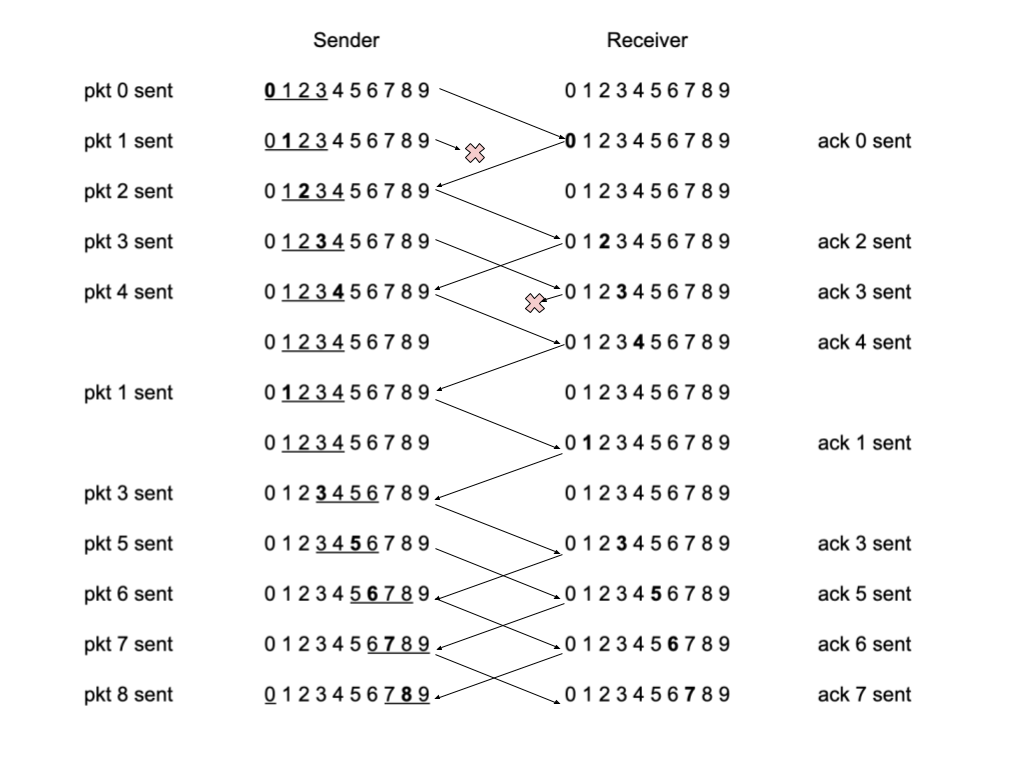
\includegraphics[width=15cm]{q1pb2}
    \item
      \begin{enumerate}[(a)]
        \item
          SR protocol must have a window size that less than or equal to half of $n$.
          This upper bound exists for the window size because of the worst case scenario:
          All of the ACK's sent by the receiver are lost. Say the window size is $w$,
          then the receiver will increment its window by $w$ places. If $w > \frac{n}{2}$,
          then the receiver's window will wrap around back to sequence number 0 again.
          This means, the receiver will confuse the sender's inevitable retransmission
          of packet 0 as a new packet rather than as a retransmission. Therefore, the
          window size $w$ must be less than or equal to half of $n$.
        \item
          GBN protocol must have a window size less than or equal to $n-1$ (i.e the
          window size must be smaller than $n$). This is because the receiver does
          not buffer any out-of-order packets. Thus in the worst case if
          all of the receiver's ACKs are lost, and the window size is $w$, the
          receiver will refuse to process any out of order packets (i.e sequence number
          that is not $w+1$). This means the sender is free to retransmit the
          previous packets and there is no concern of the receiver confusing the
          retransmitted packets as new.
      \end{enumerate}
    \item
      \begin{enumerate}[(i)]
        \item
          True. If all of the receiver's ACKs are lost, then the receiver's window
          would have advanced, while the sender's has not. Thus the sender will
          retransmit those packets and those packets will be outside of the
          receiver's window.
        \item
          True. Say the receiver's initial ACKs take a very long time to send.
          The sender will retransmit those packets, and say the receiver's second
          set of ACKs on those packets get delivered quickly, causing the sender
          to advance its window. Then the receiver's intial ACKs get delivered,
          then they fall outside of the sender's current window.
        \item
          True. The situation is exactly the same as part (ii).
        \item
          False, the receiver will not return ACK's for any packet sequence higher than
          expectedseqnum, which means there is no way the sender could advance its
          window above expectedseqnum.
      \end{enumerate}
  \end{enumerate}

\section*{Connectionless Transport}
  \begin{enumerate}[(a)]
    \item
      The checksum is the 16 bit one's complement of the the one's complement sum of
      three things:
      \begin{itemize}
        \item Pseudo header (which contains sum of the source IP, destination IP, protocol, and UDP length)
        \item UDP header
        \item Data
      \end{itemize}

      This number may be padded with zero octets at the end, if necessary, to make
      a multiple of two octets. \footnote{https://tools.ietf.org/html/rfc768}
    \item
      First convert everything to hexadecimal:
      \begin{align*}
        \text{source IP} &= \mathtt{0x44ACF5AA} \\
        \text{destination IP} &= \mathtt{0xACD90A0E} \\
        \text{length} &= \mathtt{0xE745} \\
        \text{UDP protocol} &= \mathtt{0x0011} \\
        \text{source port} &= \mathtt{0x10E1} \\
        \text{destination port} &= \mathtt{0x162E}
      \end{align*}

      Thus to calculate the 16 pseudo header, we add the source and destination IP,
      protocol and UDP length. Note that we split the IP addresses into two 16-bit
      segments:
      \[ \text{pseudo header} = \mathtt{0x44AC} + \mathtt{0xF5AA} + \mathtt{0xACD9}
       + \mathtt{0x0A0E} + \mathtt{0x0011}+ \mathtt{0xE745} = \mathtt{0x2D893} \]

      Now we can calculate the sum of the pseudo header with the UDP header and data
      (we will ignore the data since the payload is all zeros):

      \[ \text{sum} = \mathtt{0x2D893} + \mathtt{0x10E1} + \mathtt{0x162E}
      + \mathtt{0xE745} = \mathtt{0x3E6E7} \]

      Now convert the above hexadecimal into a 16 bit one's complement:
      \[ (\mathtt{0x0003} + \mathtt{0xE6E7}) \oplus \mathtt{0xFFFF} = \boxed{\mathtt{0x1915}} \]

      % https://people.engr.ncsu.edu/mlsichit/Teaching/407/index.html
      % https://stackoverflow.com/questions/30858973/udp-checksum-calculation-for-ipv6-packet
    \item
      The receiver checks for errors by computing the one's complement sum of the
      received data (which includes the checksum). If any of output bit's are 0,
      then an error is detected. The one's complement scheme makes it so that supposedly
      matching data should have an output of all 1's, making it very easy to
      computationally check.
    \item
      The checksum can fail to catch errors. The most obvious example would be that
      swapping 16-bit blocks does not change the computed checksum since summation
      is commutative. Thus, in part (b), if the source port and destination port
      were swapped (such that the destination port was 4321 and the source port
      was 5678), then the checksum would remain exactly the same!
    \item
      The theoretical maximum datagram size is 65,535 bytes since the datagram length
      field is 16 bits long.
    \item
      The size of UDP datagram cannot reach the theoretical limit in (e) because the
      length includes the IP header. The specified source and destination addresses
      are already 8 bytes each, which will detract from the maximum possible size.
    \item
      DHCP uses UDP because it is connectionless, which makes is much faster rather
      than needing to establish a 3 way handshake for every communication, which
      would be infeasible for a DHCP server sending outbound packets to many hosts.
      Furthermore, because the source does not yet have a fully configured IP
      address, this can cause problems conducting the 3 way handshake.
    \item
      Loss based congestion control have two issues, primarily revolving around the
      fact that (1) lost packets do not necessarily mean traffic congestion, and also
      (2) congestion does not necessarily mean packet loss:\footnote{https://cloud.google.com/blog/products/gcp/tcp-bbr-congestion-control-comes-to-gcp-your-internet-just-got-faster}
      \begin{itemize}
        \item
          In shallow buffers, packet loss may occur from transient traffic bursts,
          which halves the sending rate and results in less throughput than
          what the link could easily handle for most of the time
        \item
          In deep buffers, congestion may occur at deep buffers in many last-mile
          links, and this will cause a lot of delay. Loss-based congestion control
          can't account for this since no packets are lost due to the deep buffers.

      \end{itemize}
    \item
      In steady state, BBR uses the bottleneck bandwidth and round-trip propagation
      time to determine the rate and amount of packets to send through the network.
      \footnote{https://cacm.acm.org/magazines/2017/2/212428-bbr-congestion-based-congestion-control/fulltext}
    \item
      By leveraging the bottleneck bandwidth and round-trip propagation, BBR
      is able to ensure that the bottleneck runs at 100\% utilization, and
      also guarantees there is enough data to "prevent bottleneck starvation
      but not overfill the pipe". In otherwords, the bottleneck ultimately
      determines the congestion level of the network, and by pacing packets
      to be exactly what the bottleneck can handle would maximize the number
      of packets sent without causing overflowing congestion.\footnote{Ibid.}
  \end{enumerate}

\section*{Connection-Oriented Transport}
  \begin{enumerate}[(a)]
    \item
      If Host Y receives the first segment normally, the ACK will return the number
      number 100. If Host Y receives the second segment first, the ACK will return the
      number 80.
    \item
      \begin{enumerate}[(i)]
        \item
          From the table below, the EstimatedRTT is $\boxed{89.99}$ ms.

          \begin{table}[H]
            \begin{tabular}{lllll}
            \hline
            Time & SampleRTT & EstimatedRTT &  &  \\
            \hline \\
            1    & 120       & 120          &  &  \\
            2    & 25        & 110.5        &  &  \\
            3    & 35        & 102.95       &  &  \\
            4    & 40        & 96.66        &  &  \\
            5    & 30        & 89.99        &  & \\
            \hline
            \end{tabular}
          \end{table}

          SampleRTT5 has the largest impact on the EstimatedRTT because the alpha
          value is 0.1, giving 9 times more weight to the previous estimate
          than to the current sample. This combined with the very few number of samples
          makes a disproportionate amount of weight added to prior estimates.
        \item
          Given n SampleRTT's, with $\text{SampleRTT}_1$ being the most recent one:
          \[ \text{EstimatedRTT} = \left( \alpha \sum^{n-1}_{i=1} (1 - \alpha)^{i-1} \text{SampleRTT}_i \right) + (1 - \alpha)^{n-1} \text{SampleRTT}_n \]

          Given $\alpha = 0.1$:
          \[ \text{EstimatedRTT} = \left( 0.1 \sum^{n-1}_{i=1} 0.9^{i-1} \text{SampleRTT}_i \right) + 0.9^{n-1} \text{SampleRTT}_n \]
      \end{enumerate}
    \item
      The information in the last packet when establishing a connection is the
      client's ACK for the server's initial sequence number. This packet is necessary
      as a TCP connection is meant to provide for bi-directional communication, and thus
      without it, the server hasn't finished synchronizing its initial sequence number
      with the client  (it hasn't been ACK'ed yet). This prevents the server from sending
      communication over the connection, and hence breaks the bidirectionality of
      a TCP connection.
    \item
      In the client's first packet to the server, it will set the SYN bit in the flag
      field to be 1. Additionally, the sequence number field will also be set
      to the client's choosing.

      In the server's return packet to the client, the SYN bit in the flag field
      is also set to 1. The acknowledgement field in the header is set to be
      the client's ISN + 1. The sequence number field in the header is also
      set to the server's choosing.

      In the third packet of the handshake (client's second packet to the server),
      the acknowledgement field in the header is set to be the server's ISN + 1.
      The SYN bit in the flag field is also set to 0.
    \item
      The FIN flag is used to close a connection. The other end sends an acknowledgement
      to complete the closure.
    \item
      Only two handshake packets are needed to establish a unidirectional, reliable
      connection-oriented protocol. This is because only A's ISN needs to be
      synchronized across the two servers in order for B to reliably receive
      A's messages. The process would look like the following: A will send a SYN packet
      with its ISN to B, and then B needs to respond with an ACK packet to A. Now
      A knows that its can reliably send messages to B starting at that ISN,
      and communciation and henceforth begin.
    \item
      Only two steps are needed to close the connection started by A, since only
      one set of buffers and resources needs to be deallocated. It would just be
      one FIN packet sent by the initiator of the closure, and an ACK packet
      returned.
    \item
      The TCP sender only maintains the smallest sequence number of a transmitted
      but unACK'ed byte as well as the sequence number of the next byte to be send,
      making the sender side look a lot like the GBN protocol.
    \item
      On the receiver's side, many TCP implementations will correctly buffer
      out-of-order segments that are received, which is similar to a Selective
      Repeat behavior. On the sender's side, retransmission also works like
      Selective Repeat, where it would only retransmit specific retransmit segments that
      are timed out.
    \item
      Just using NAK's is not sufficient to allow A to tell the status of the segments.
      In the case where B is only expecting seg1, and say receives seg1 and seg2
      (this means seg3 and seg4 dropped). B will not respond with any NAK's,
      since it doesn't know that it was supposed to receive seg3 and seg4, and B's
      lack of response makes A believe that all of the segments were successfully sent,
      when in reality 2 of the segments actually dropped.
    \item
      The super fast retransmission does not work well in situations where multiple
      packets are lost successively. For example, let's say seg2, seg3, seg4, and seg5 were
      all dropped (so the packet status is 100001). The receiver will send an ACK for
      seg1 after receiving seg1. Then once the receiver gets seg6, it will do
      one of the following:
      \begin{itemize}
        \item
          In the super fast retransmission protocol, the receiver will return a
          duplicate ACK for seg1 since it received an out-of-order segment with
          a higher than expected sequence number (seg6). This would be a duplicate ACK
          on the sender's end, so it would send seg2, which the receiver would
          ACK once it receives. Then the sender's timer for seg3, seg4, seg5 and
          seg6 would expire and it would retransmit those packets. The receiver receives
          all of those packets and then ACK's all of them accordingly.
        \item
          In the NAK protocol, the receiver will send a NACK for segments 2 through 5,
          since it received segment 1 and segment 6 (and knows that it is out of order).
          The sender will receive the NACK, and then retransmit segments 2 through 5.
          The receiver will receive them and ACK all of them.
      \end{itemize}

      From the two cases above, the NACK protocol improved overall performance because
      it retransmitted fewer segments (it did not need to retransmit segment 6 twice
      as it did in the super fast retransmission case), and also it started
      retransmission earlier for segments 3 through 5 -- i.e when it received the NACK
      rather than when it waited for the timer to expire in the super fast retransmission
      case.
    \item
      The above case worked because propagation delay is larger than transmission
      delay, which means that the sender would likely have sent all of the segments
      out before hearing any response from the receiver. This makes multiple sequential
      dropped segments even more costly because the sender was unable to receive
      feedback as it was sending each individual segment (and thus ultiamtely
      relying on the timer to figure out seg3 through seg5 were dropped).

      The above case is unlikely and limited because it required the propagation delay
      to be so much larger than transmission delay that all of the sender's segments
      were enroute by the time the first response reached the sender. The above
      case also assumed that NACK's can't be dropped enroute, and also ignores cases when
      the later segments were dropped (without the receiver's knowledge that
      it was supposed to receive them)
  \end{enumerate}

\section*{Methods of Congestion Control and avoidance}
  \begin{enumerate}[(a)]
    \item
      (1) Flow control prevents the receiver's buffer from being overwhelmed
          (sender bears the responsibility),
          while congestion control prevents the network (router buffers) from
          being overwhelmed (transport layer bears responsibility).

      (2) The point of congestion control is to ensure everyone on the network
          has fair access to the resources, while the point of congestion
          control is ensure smooth communication between two people
    \item
      This would technically work but be terribly inefficient. Congestion control
      would never replace flow control because the premise of congestion control
      is that the sender is unsure how congested the networks are (how many other
      people are on the network, how heavy is their usage, what is the state of
      the router buffers), and thus attempts to maximize the amount of packets
      sent without overloading the network. However, when just sending to another
      person, their buffer size is known, and the amount of remaining space
      on the buffer is also known. Thus, there is no need to optimize the maximum
      throughput, and instead the known number can just be used.

      Furthermore using loss controlled flow control is also fundamentally inefficient
      because retranmission of the lost packets is required, when compared to a flow
      control algorithm that can guarantee no packet losses on the client's end.
    \item
      During Fast Recovery, packet retransmission occurs when the sender receives
      3 duplicate ACKs. It then sends half the number of packets that it previously
      sent (congestion window cut in half).

      During normal recovery, packet
      retransmission occurs when the sender witnesses a timeout occuring for a
      packet that it sent. It then cuts its congestion window to 1 MSS.
    \item
      Neither fast nor normal recovery definitely mean a packet was lost. This is
      because different packets may take different routes based on the state
      of the congestion, and hence packets may arrive out of order, causing 3
      ACK's to go out before the missing packet arrives. Timeouts may also
      occur without packet loss due to network congestion.
    \item
      Congestion window is halved during fast recovery. The window is set to
      equal to 1 MSS during normal recovery.
    \item
      Relying on too few duplicate ACK's does not signal strong confidence that
      the packet was lost (because packets can be re-ordered), thus retransmitting
      in this case makes it likely that duplicate work is being done (as the packet
      is unlikely to have been lost).

      Relying on too many duplicate ACK's waits beyond a reasonable measure of
      confidence that the packet was lost, effectively wasting time before
      starting the retransmission process.
    \item
      In networks where the buffer sizes and RTT's are fairly homogenous, Vegas
      would perform better as it would not be forced to wait for packets to be
      lost (which would require retransmission), and can take preventative efforts
      to scale back.

      However, in situations where the network is very heterogenous, Reno may
      be better as packets can be routed differently based on congestion levels
      and one high RTT for a packet does not necessarily mean the network is
      on the brink of congestion collapse.
    \item
      My answer would be different, because TCP Vegas is based on the premise of
      RTT rather than packet loss. Looking for duplicate ACK's is a measure of
      confidence of packet loss rather than RTT, and thus a completely different
      measure than what Vegas is using.
    \item
      A Vegas network with a Reno network would not be fair, as the linear
      increase and linear decrease fails to move the connection throughout to
      the equal bandwidth share (the multiplicative decrease is the key that decreases
      the throughput proportionally to the equal bandwidth share).

      For streaming videos, I would not use Vegas -- I would still use UDP, as
      UDP does not abide by fairness congestion control and videos do not want
      their transmission rate to be throttled.
    \item
      \[ (6, 14) \text{ and } (15, 26) \]
    \item
      32 MSS
    \item
      A packet was lost by detecting 3 duplicate ACKs and fast recovery was implemented
      (congestion window halved). This event definitely indicates that at least one
      packet was sent, as the receiver only sends a duplicate ACK when receiving an
      out of order segment.
    \item
      A packet was lost due to a timeout, thus normal recovery occured (where the
      congestion window was set to 1 MSS)
    \item
      No this does not definitely indicate that the network discarded a packet.
      Network congestion could have delayed the packet enroute such that the
      sender's timer expired before it arrived.
    \item
      The threshold immediately before round 27 is 20 MSS (because it is half
      the congestion window size at the previous loss event, which was at 40).

      Round 28 is at 1 MSS. After round 28 the congestion window starts at 2 (round 29).
      Assuming no losses, the congestion window will grow to 4, then 8, then 16,
      then exceed the previous threshold on round 33.

      Assuming that the packets are able to be put on the link in quick succession
      (i.e negligible time difference between when the packets are put on the link),
      each round takes one RTT to complete. It will take four rounds, and thus
      4 RTT's, or \textbf{400 ms} before the congestion window size reaches the previous threshold.
  \end{enumerate}
\end{document}
